\chapter{Redox: Pathway Exploration}

\section{Purpose}
The purpose of this chapter is to describe Redox, a web application designed to run offline or deployed online, that is used to visualize, explore, and analyze large sets of biochemical network pathways.
Redox was developed with the scientists at Arzeda Inc (\url{http://arzeda.com/}) as the primary end users and source of feedback.
However, Redox is an example of modular design using the yeoman build tools.
Additional data controllers and templates may also be easily added to extend compatibility with input sources and custom layouts.

\section{Motivation}
\subsection{Metabolic engineering of microorganisms can lead to new ways to produce valuable commodities.}
\subsection{The space of possible potential candidate pathways is extremely large.}
KEGG
Biochemical reactions 9,647
Metabolites and other small molecules 17,257
\subsection{Semi-automated pathway selection requires curation.}


\section{Solution}
\subsection{}
\subsection{}
\subsection{}

\begin{figure}
  \centering
  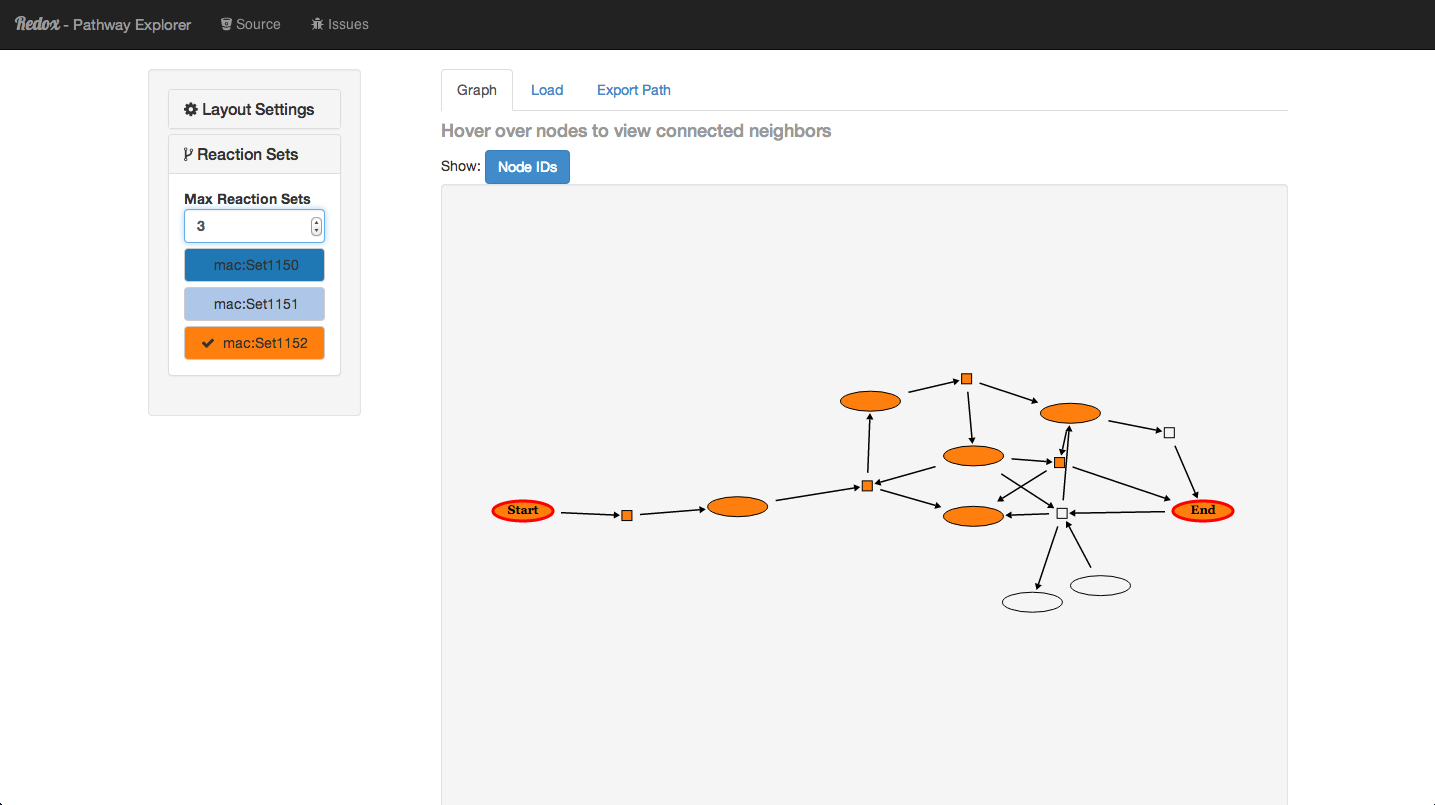
\includegraphics[width=\textwidth,natwidth=610,natheight=642]{images/redox-ui.png}
  \caption{Pathway exploration using Redox}
  \label{Figure:redox}
\end{figure}


\begin{figure}
  \centering
  \caption{Swapping layout templates.}
  \label{Figure:redoxLayouts}
\end{figure}



\section{Implementation}
\subsection{}
\subsection{}
\subsection{}
